\resizebox{0.98\linewidth}{!}{%
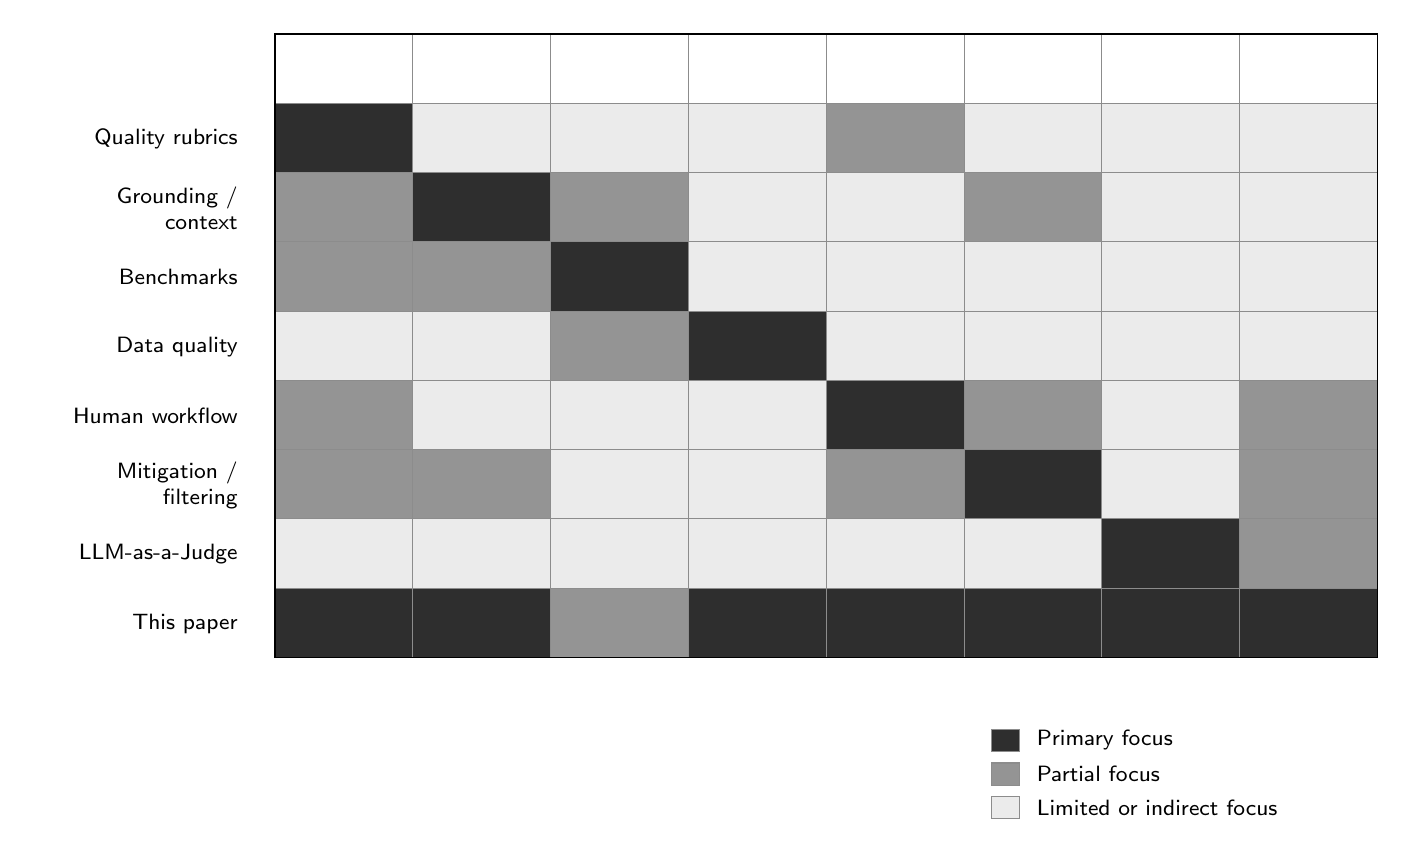
\begin{tikzpicture}[
  font=\sffamily\footnotesize,
  header/.style={font=\sffamily\bfseries\footnotesize, align=center, text width=2.05cm},
  rowlabel/.style={font=\sffamily\footnotesize, align=right, text width=2.55cm},
  celltext/.style={font=\sffamily\scriptsize, align=center},
  legendtext/.style={font=\sffamily\footnotesize, anchor=west},
]

\definecolor{primaryFocus}{gray}{0.18}
\definecolor{partialFocus}{gray}{0.58}
\definecolor{limitedFocus}{gray}{0.92}
\definecolor{gridLine}{gray}{0.55}

\def\cellw{1.75}
\def\cellh{0.88}
\def\xstart{3.0}
\def\ystart{0}

% Column headers.
\node[header] at (3.875, 0.55) {Quality};
\node[header] at (5.625, 0.55) {Grounding};
\node[header] at (7.375, 0.55) {Benchmark\\realism};
\node[header] at (9.125, 0.55) {Data\\validity};
\node[header] at (10.875, 0.55) {Workflow\\value};
\node[header] at (12.625, 0.55) {Mitigation};
\node[header] at (14.375, 0.55) {Evaluator\\validity};
\node[header] at (16.125, 0.55) {Decision\\level};

% Row labels.
\node[rowlabel] at (1.25, -0.45) {Quality rubrics};
\node[rowlabel] at (1.25, -1.33) {Grounding /\\context};
\node[rowlabel] at (1.25, -2.21) {Benchmarks};
\node[rowlabel] at (1.25, -3.09) {Data quality};
\node[rowlabel] at (1.25, -3.97) {Human workflow};
\node[rowlabel] at (1.25, -4.85) {Mitigation /\\filtering};
\node[rowlabel] at (1.25, -5.73) {LLM-as-a-Judge};
\node[rowlabel] at (1.25, -6.61) {This paper};

% Helper macro: x index, y index, color.
\newcommand{\focuscell}[3]{%
  \pgfmathsetmacro{\x}{\xstart + (#1) * \cellw}%
  \pgfmathsetmacro{\y}{\ystart - (#2) * \cellh}%
  \draw[draw=gridLine, line width=0.35pt, fill=#3] (\x,\y) rectangle ++(\cellw,-\cellh);%
}

% Header row cells.
\foreach \c in {0,...,7} {\focuscell{\c}{-1}{white}}

% Row 1: Quality rubrics.
\focuscell{0}{0}{primaryFocus}
\focuscell{1}{0}{limitedFocus}
\focuscell{2}{0}{limitedFocus}
\focuscell{3}{0}{limitedFocus}
\focuscell{4}{0}{partialFocus}
\focuscell{5}{0}{limitedFocus}
\focuscell{6}{0}{limitedFocus}
\focuscell{7}{0}{limitedFocus}

% Row 2: Grounding/context.
\focuscell{0}{1}{partialFocus}
\focuscell{1}{1}{primaryFocus}
\focuscell{2}{1}{partialFocus}
\focuscell{3}{1}{limitedFocus}
\focuscell{4}{1}{limitedFocus}
\focuscell{5}{1}{partialFocus}
\focuscell{6}{1}{limitedFocus}
\focuscell{7}{1}{limitedFocus}

% Row 3: Benchmarks.
\focuscell{0}{2}{partialFocus}
\focuscell{1}{2}{partialFocus}
\focuscell{2}{2}{primaryFocus}
\focuscell{3}{2}{limitedFocus}
\focuscell{4}{2}{limitedFocus}
\focuscell{5}{2}{limitedFocus}
\focuscell{6}{2}{limitedFocus}
\focuscell{7}{2}{limitedFocus}

% Row 4: Data quality.
\focuscell{0}{3}{limitedFocus}
\focuscell{1}{3}{limitedFocus}
\focuscell{2}{3}{partialFocus}
\focuscell{3}{3}{primaryFocus}
\focuscell{4}{3}{limitedFocus}
\focuscell{5}{3}{limitedFocus}
\focuscell{6}{3}{limitedFocus}
\focuscell{7}{3}{limitedFocus}

% Row 5: Human workflow.
\focuscell{0}{4}{partialFocus}
\focuscell{1}{4}{limitedFocus}
\focuscell{2}{4}{limitedFocus}
\focuscell{3}{4}{limitedFocus}
\focuscell{4}{4}{primaryFocus}
\focuscell{5}{4}{partialFocus}
\focuscell{6}{4}{limitedFocus}
\focuscell{7}{4}{partialFocus}

% Row 6: Mitigation/filtering.
\focuscell{0}{5}{partialFocus}
\focuscell{1}{5}{partialFocus}
\focuscell{2}{5}{limitedFocus}
\focuscell{3}{5}{limitedFocus}
\focuscell{4}{5}{partialFocus}
\focuscell{5}{5}{primaryFocus}
\focuscell{6}{5}{limitedFocus}
\focuscell{7}{5}{partialFocus}

% Row 7: LLM-as-a-Judge.
\focuscell{0}{6}{limitedFocus}
\focuscell{1}{6}{limitedFocus}
\focuscell{2}{6}{limitedFocus}
\focuscell{3}{6}{limitedFocus}
\focuscell{4}{6}{limitedFocus}
\focuscell{5}{6}{limitedFocus}
\focuscell{6}{6}{primaryFocus}
\focuscell{7}{6}{partialFocus}

% Row 8: This paper.
\focuscell{0}{7}{primaryFocus}
\focuscell{1}{7}{primaryFocus}
\focuscell{2}{7}{partialFocus}
\focuscell{3}{7}{primaryFocus}
\focuscell{4}{7}{primaryFocus}
\focuscell{5}{7}{primaryFocus}
\focuscell{6}{7}{primaryFocus}
\focuscell{7}{7}{primaryFocus}

% Outer border.
\draw[draw=black, line width=0.6pt] (\xstart,0.88) rectangle ++(8*\cellw,-9*\cellh);

% Legend.
\draw[fill=primaryFocus, draw=gridLine] (12.1,-7.95) rectangle ++(0.35,-0.28);
\node[legendtext] at (12.55,-8.09) {Primary focus};
\draw[fill=partialFocus, draw=gridLine] (12.1,-8.38) rectangle ++(0.35,-0.28);
\node[legendtext] at (12.55,-8.52) {Partial focus};
\draw[fill=limitedFocus, draw=gridLine] (12.1,-8.81) rectangle ++(0.35,-0.28);
\node[legendtext] at (12.55,-8.95) {Limited or indirect focus};

\end{tikzpicture}%
}
